\newif\ifbook \booktrue

%@- This is so lgrind will get along with makeindex.

\ifbook
	\chapter{C} \label{c_crash}
\else
	\long\def\comment#1{}
	\documentclass[12pt]{article}
	\usepackage{amsfonts}  %for mathbb
	\setlength{\topmargin}{-0.5cm}\setlength{\textheight}{8.6in} 
    \setlength{\oddsidemargin}{0in} 
    \setlength{\textwidth}{6.1in} 

	\usepackage[nolineno,noprocindex]{lgrind}

    %indexing:
    \usepackage{multicol, makeidx}
    \makeindex
    \def\ind#1{\index{#1}#1}
    \def\cind#1{\index{#1@\cinline{#1}}\cinline{#1}}
    \def\cindex#1{\index{#1@\cinline{#1}}}
    \def\ff#1{#1 {\it ff}} %e.g. \index{pointers|ff}

	\begin{document}
	\title{A crash course in C}
	\author{B Klemens}
	\maketitle


Dear Reader:\\
This is a crash course in C intended for a book on statistics using the
GNU Scientific Library (the GSL).  Since it basically stands alone as a
C tutorial, I offer it to you as such. I haven't edited this from
its chapter form, so it refers to sections outside of this tutorial,
for which I apologize. Although written for researchers programming
statistical tests, it will be useful to any of you who have done some
programming in a scripting language and would like to get to know C.

\vskip 1cm

\section{C}
\fi

\comment{The next bit defines the code figures.
I'm using lgrind now; it's pretty standard.
The first argument to codefig will be
both the name of the file and the label the figure will have; the 
second argument will be caption for the figure.


%The deprecated lgrind version.
%\long\def\codefig#1#2{
%	\begin{figure}
%	\hrule\vskip4pt
%	\input sources/#1.tex
%\lstinputlisting[language=C, showstringspaces=false, basicstyle=\scshape,breaklines=true,prebreak=-]{sources/#1.c}
%	\hrule
%
%	\caption{#2}\label{#1}
%	\end{figure}
%}
}

\long\def\codefigbyinclusion#1#2#3{
	\begin{figure}
	\hrule\vskip4pt
	#1
	\hrule

	\caption{#3}\label{#2}
	\end{figure}
}

%\long\def\codefig#1#2{\lagrind{sources/#1.tex}{#2}{#1}}


This chapter will bring you up to speed on C.  
My hope with this chapter is both to discuss where to put your semicolons
and how things are generally done in C. Don't feel compelled to memorize
everything here (using \cinline{malloc} three times in a sentence, for
example), since the manual is always there for you to read.  It is not
a comprehensive tutorial: GNU C recognizes 32 key words and this book
will only use 17 of them. For example, we won't be using bit-shifting
operators, so I'm not going to tell you what they are here.  If you want
more details about any of the points I mention here, just type \binline{C
tutorial} into your favorite search engine; since this is C and not a
proprietary, specialized language, you will have a few hundred hits to
choose from. 

The first part (up to Section \ref{pointers})
is all about functions, which are mostly self-contained pieces of code,
but which call and are called by other functions. I will discuss how
those functions are declared and defined, where to put them, and how the
computer goes about keeping track of functions that call functions that
call other functions. The second part, pointers, discusses C's method
of circumventing this neat functional structure by directly handling
parts of the computer's memory without C's automatic memory handling
getting in the way.

\subsection{The tools} 
Most stats packages are built around a single window that includes a
space for you to type commands and a space for output to be displayed.
They also give you the option of putting all of your commands into a
text file, and then the package reads the text file and displays output.

First, C works almost entirely in the paradigm of putting commands in a
text file and then running the text file all at once. Second, since
C is an open standard rather than a product from a single company, there
are hundreds of programs available to help you write the text file and
produce the output. Your problem is not in finding such tools, but in
choosing which you will use.

The first element you will need is a compiler. If you are using
a UNIX-like system, you probably already have \cind{gcc} on your
computer. Try typing \binline{cc} on your command line; if you get an
error like ``command not found'', then you will need to get a compiler,
but an error like ``no input files'' means that a compiler was found
and awaits input. Windows and Mac OS do not ship with a compiler; if you
are using a computer customized by your university or company computing
department, check the usual application folders.

On top of the compiler, you will need a debugger like gdb, the standard
libraries, the GNU Scientific Library (GSL) and SQLite.  The easiest
way to get all of these disparate tools is via a package manager. If
you are using a UNIX-like system, you are probably already familiar with
your package manager (Red Hat Package Manager and Debian's Apt are the
most popular).

If you are using Windows, you have two options. One is to get
Mingw, which provides a compiler and not much else. It has its
own installation program. The other option is to get Cygwin.
It is free, has a pleasant package-oriented
installation program, and provides an entire UNIX subsystem, with the
attendant compilers, editors, and so on. Be sure to select gcc, gdb,
the GSL, and SQLite under the development subsection in the installation.

Mac OS X users will be using the terminal (typically found in the
accessories subfolder of the Applications folder) to do most of the
work below. The package manager of choice is Fink, which can easily be
found and installed online.

Herein, I will assume that you have a working copy of \cinline{gcc},
\cinline{gdb}, et cetera, and it is on the search path for executables
on your system. If this is not the case, then abundant help is available,
either from your local computer guru or from your favorite search engine.

If you will be using Apophenia or would like further notes on
installation, see the Setup section of the online reference, at
\url{http://apophenia.info/doc}.

\paragraph{IDEs} \index{IDE} \index{integrated development environment}
Broadly, you have the choice of two paradigms in which to work. The
first is the integrated development environment (IDE). This is an
all-in-one environment comparable to a multiwindow stats package, with
one window for your program, one for compilation, one for output, et
cetera.  
Popular choices include Dev-C++ or Eclipse. Many other IDEs of varying
quality are available for any graphically-oriented operating system.

The other option is via the command line. Since you are certainly using
a system that supports multiple windows,\footnote{Even if you are
dialing in to a server's single-window terminal, you can either dial in
twice, or use \binline{screen} to multiplex the window.} 
you are basically using your operating system as an IDE.
In this paradigm, you will probably have one window that is dedicated to
a text editor with your code, and another window for compilation,
debugging, and output.



\paragraph{Text files} C programs are files of text, and all of your work
will be manipulations of text, so it is in your long-run best interest to
get a good \ind{text editor}. At the very least, you will get error messages
listing line numbers, so if your text editor can't tell you which is
line 105, you will need to get a new one.

The two most popular are \ind{EMACS} and \ind{vi}. EMACS is better for
people who prefer to have everything under one roof---it is often billed
as an IDE---while vi is better for the minimalists and touch typists. Both
involve a learning curve, meaning that they will be difficult to use at
first, will require reading the manual, and will in the long run save
you hours over using simpler text editors such as those typically
included with IDEs. Some implementation of both is available for all
computer types, and you are encouraged to start learning one or the other
now. If neither suits your fancy, there are literally hundreds of others
to choose from. That said, I will assume you have a good text editor
(by your personal definition of \airq{good}), and will turn to the text you
will be writing with it.
\ifbook \else 
	\input why_c.tex
\fi
\paragraph{An outline} The remainder of this chapter dives in to the
syntax and form of C. The first half starts small, on individual
lines, and then covers means of organizing blocks of code in
functions, and then organizing blocks of functions in file modules.
Section \ref{fncontents} covers what individual lines of code can do;
this section will probably be the most familiar to one well-versed with
the typical stats package.  Section \ref{declaring} covers the nouns
of the language: the variables. Section \ref{functional} introduces the
verbs: the functions. The execution of a C program consists of evaluating
functions, which means that most of the work you will be doing will be in
writing good functions, so this section will discuss some of the ideas
behind functional form.  Section \ref{compilation} will discuss how to
use your compiler to produce executable programs, assembling together
functions from disparate locations. Section \ref{pointers} covers
\airq{pointers}, a C-specific means of handling computer memory that
complements C's means of handling functions and large data structures. The
remainder of the chapter covers additional topics such as the debugger
and assorted idiosyncrasies and conveniences of C syntax.


\comment{
\subsection{An opening sample}
To get the conversation started, here is a complete sample program.
The program writes down a vector of numbers, and prints their mean.
\label{initialsample}
\begin{lstlisting}[numbers=left, numberstyle=\scshape]
#include <stdio.h>

int main(void){
    float data[] = {2,4,8,16,32};
    int data_ct = 5;
    int i;
    float mean = 0;
    for (i=0; i< data_ct; i++){
        mean += data[i];
    }
    mean /= data_ct;
    printf("The mean is %g.\n", avg);
    return 0;
}
\end{lstlisting}
Line 1 is a call to an external header file, and will
be discussed in Section \ref{headers}. 

Line 3 is a function header. A C program does only two things: allocate
variables and run functions.  You will see time and time again that the
focus in writing good code is not about writing out lengthy procedures, but 
writing small functions that do one thing well. The entire program as
such is just a function named \cinline{main}. Since functions typically
output a value, and line 13 shows that this function returns zero.

Inside this function, the first thing we do is allocate variables. As in
Section \ref{declaring}, all variables have to be declared. Line four
declares an array of five data points, and lines 5--7 declare scalars.

Lines 8--10 are a \cinline{for} loop. Line 8 may seem ornery, but
Section \ref{forloops} will explain that it simply takes the variable
\cinline{i} through the indices of the \cinline{data} vector. 

Line 9 increments  the value of \cinline{avg} by the value of the
\cinline{i}th element of the \cinline{data} array. In R, this would be
written as \cinline{mean <- mean + data[i]}, and similarly in other
languages. 

By line 11, \cinline{mean} has the sum of all of the elements of the
vector, and line 11 divides the mean by the number of data points to
produce the actual mean. 

Some stats packages print out every step of the process; C is much
quieter and will only speak when asked.  Line 12 actually prints out
the value of the mean. Its syntax is explained on page \pageref{printf}.

If you are familiar with the commands of the typical stats package, the
program should have some familiar and unfamiliar components. The odd
syntax, such as the line about the \cinline{for} loop, is simply a
question of getting used to a new language. For many scriptwriters,
the fact that everything happens in the context of a function is often
a new means of thinking about writing a program. It is not the most
direct means, but by the end of this chapter you should see its immense
benefit. The variable declarations may be a bit tedious, but they are
easy enough.
}

\section{Lines} \label{fncontents}

The story begins at the smallest level: a single line of code. Most of
the work on a single line of code will be familiar to anyone who has
written programs in any lanugage, including instructions like assignments,
basic arithmetic, if-then conditions, and loops. For such common
programming elements, learning C is simply a question of the details
of syntax. Also, C is a \airq{typed} language, meaning that you will
need to specify whether every variable and function is an integer,
a real, a vector, et cetera. Thus, many of the lines will be simple
type declarations.

\subsection{Assignment} \index{arithmetic} \index{assignment|see{=}} \index{=}
Most of the work you will be doing will be simple assignments:\\
\cinline{ratio = a / b;}\\
will find the value of \cinline{a} divided by \cinline{b} and put the
value in \cinline{ratio}. Notice that there is a semicolon at the end of
the line; you will need a semicolon at the end of everything but the few
exceptions I mention below.\footnote{The number one cause of compiler
complaints like ``line 41: \ind{syntax error}'' is a missing semicolon on line 40.} All of the usual operations work: \cinline{+
- / *}, and so do some of the more obscure ones, like \cinline{a \% b}
for $a$ mod $b$. \index{modulo|see{\%}} \index{\%}

\subsection{Incrementing}\index{incrementing} It is incredibly common to have an operation of the form \cinline{a = a + b;}---so
common that C has a special syntax for it: \cinline{a += b;} This is slightly less readable, but involves less
redundancy. All of the above arithmetic operators can take this form, so each of the following lines show two
equivalent expressions: \\
\begin{lstlisting}
a -= b;     a = a - b;
a *= b;     a = a * b;
a /= b;     a = a / b;
a %= b;     a = a % b;
\end{lstlisting}

Finally, the most common operation among these is incrementing or decrementing by one, and so C offers the
following syntax for still less typing:\footnote{There is also the pre-increment form, \cinline{++a} and
\cinline{--a}. Pre- and post-incrementing differ only when they are being used in situations that are bad style and should
be avoided. Leave these operations on a separate line and stick to whichever form looks nicer to you.} \\
\begin{lstlisting}
a++; /*is equivalent to*/ a = a + 1;
a--; /*is equivalent to*/ a = a - 1;
\end{lstlisting}



\subsection{Conditions} 	
\label{forloops} \index{conditionals} \index{boolean expressions} \index{logical expressions} 
\cindex{<} \cindex{>} \cindex{==}
Another set of operators are comparison and logical operators, such as \cinline{(a $>$ b)},
\cinline{(a $<$ b)}, or \cinline{(a == b)}. All of these evaluate to either a one or a zero, depending on whether the
comparison is true or false. Notice that last one, comparison for equality, involves {\sl two} equals
signs in a row. One equals sign \cinline{(a = b)} will assign the value of \cinline{b} to the variable \cinline{a}, which is not what
you had intended. gcc will warn you in most of the cases where you are
probably using the wrong one, and you should heed its warnings. \airq{Greater than or equal to} is \cinline{(a $>=$ b)}, and \airq{less than or equal to} is \cinline{(a $<=$ b)}.

Logical operations have similar definitions: \cindex{\&\&} \cindex{"|"|} \index{and|see{\&\&}}
\index{or|see{$"|"|$}} \index{not|see{"!}} \index{"!}
\airq{And} is \cinline{(a \&\& b)}; \airq{or} is \cinline{(a || b)}; \airq{not \cinline{a}} is \cinline{(!a)}.
The \cinline{\&\&} and \cinline{||} operations have a convenient feature: if \cinline{a} is sufficient to determine whether
the entire expression is true, then it won't bother with \cinline{b} at all. For example [just ignore the \cinline{\#include} lines for now]:
\begin{lstlisting}
#include <math.h>    //sqrt
((a < 0) || (sqrt(a) < 3))
\end{lstlisting}
will always work: if \cinline{a} is less than zero, then the evaluation
of the expression is done (it is true), so the square root won't have
to be calculated, avoiding any square-root-of-a-negative error. 
[The \cinline{sqrt()} function isn't a fundamental part of C---you
need to include an external header to get the declaration; see below.]

Why all the parentheses? First, parentheses indicate the order of
operations, as they do in pencil-and-paper math. Since all comparisons
evaluate to a zero or a one, both \cinline{(~(a $>$ b) $||$ (c $>$ d) )}
and \cinline{(a $>$ (b $||$ c) $>$ d)} make sense to C. You probably meant
the first, but unless you have the order-of-operations table memorized,
you won't be sure which of the two C thinks you mean by \cinline{(a $>$
b $||$ c $>$ d)}.\footnote{The order-of-operations table is available
online, but the reader is encouraged to not look it up. Most
people remember only the basics like how multiplication/division comes before
addition/subtraction; if you rely on the order-of-operations table
for any other ordering, then you will merely be sending future readers
(perhaps yourself) to check the table.}

Second, you will occasionally use these in normal arithmetic or an assignment. This line:
\begin{lstlisting}
b = c == d;
\end{lstlisting}
is correct: if \cinline{c} equals \cinline{d}, then \cinline{b} will be one, otherwise \cinline{b} will be zero. But
it is visually a bit off-putting, and in a more complex example gets very confusing. Using
\begin{lstlisting}
b = (c == d);
\end{lstlisting}
makes this ornery statement a touch more readable.

The primary use of these conditionals is in flow control: causing
the program to repeat some lines until a condition is true, or execute some lines only if a condition is
false.  In all of the cases below, you will need parentheses around the conditions, and if you forget,
you will get a confusing compiler error.

\subsection{If-then-else statements} Here is the syntax for conditional evaluations: \cindex{if}

\begin{lstlisting}
#include <math.h>
if (a > 0)
    { b = sqrt(a); }
else 
    { b = 0; }
\end{lstlisting}
So if \cinline{a} is positive, then \cinline{b} will be given the value of \cinline{a}'s square root; if \cinline{a} is
zero or negative, then \cinline{b} is given the value zero. Notice all those brackets: the condition to be
evaluated is always in parentheses following the if statement, and there should be curly brackets around
the part that will be evaluated if the condition is true, and around the part that will be evaluated if
the condition is false. You can exclude the curly braces if they surround exactly one line, but this
will at some point confuse you and cause you to regret leaving them out.
You can exclude the \airq{else} part if you don't need it (which is common, and much less likely to confuse you).

Also, notice the semicolons, which come after every line in the program that is not flow control. The \cinline{if (a $>$ 0)} statement doesn't do anything by itself, just direct flow, so there must be no semicolon following
it.\footnote{If you do put a semicolon after an \cinline{if} statement
(e.g., \cinline{if (a $>$ 0);}, then your \cinline{if} statement will
execute the null statement \cinline{/*do nothing*/;} if true. Your
compiler will warn you of this.}


\subsection{Loops} There are three types of loops, and they are slightly redundant. The simplest is a while
loop. Here is a while loop to print \airq{hello} on the screen five times: \index{loops} \cindex{while}

\begin{lstlisting}
#include <stdio.h>
int i = 0;
while (i<5){
    printf("Hello.\n");
    i++;
}
\end{lstlisting}

The interpretation is rather straightforward: while the expression
in parentheses is true (mustn't forget the parentheses), execute the
instructions in brackets.

Cases like the example above, where we have a counter which we increment,
are so common that they have their own special syntax. The following
\cind{for} loop is exactly equivalent to the while loop above:

\begin{lstlisting}
#include <stdio.h>
int i;
for (i=0; i<5; i++){
    printf("Hello.\n");
}
\end{lstlisting}

Comparison with the above tells us when the three subelements in the
parentheses are evaluated: the first part is evaluated before the
loop runs; the second part is tested at the beginning of each
iteration of the loop; the third part is evaluated at the end of each
loop. After the section on arrays, you will be very used to the 
\cinline{for (i=0; i<limit; i++)} form, and will recognize it to mean `step
through the array'.

Finally, if you want to guarantee that the loop will run at least once, you can use a \cind{do-while} loop (with a semicolon after the \cinline{while}):

\begin{lstlisting}
#include <stdio.h>
int i = 0;
do {
    printf("Hello.\n");
    i++;
} while (i<5);
\end{lstlisting}
In this case, the \cinline{do-while} loop here is equivalent to the
\cinline{while} and \cinline{for} loops above. But say that you want to
iteratively evaluate a function until it converges to within $1\times
10^{-3}$.  The form would be something like:
\begin{lstlisting}
#include <stdio.h>
do {
    error = eval_fn();
} while (value>1e-3);
\end{lstlisting}
Naturally, you would want to run \cinline{eval\_fn()} at least once.

\subsection{Comments} \index{commenting code|(}
Put a long block of comments 
at the head of a file and at the head of each function to describe what
the file or function does, using complete sentences. Describe what the
function expects to come in, and what the function will put out.
\begin{verbatim}
/* Long comments begin with a slash-star,
   continue as long as you want, and end 
   at the first star-slash:   
   */
\end{verbatim}

The primary audience of your comment should be you, six months from
now. When you are shopping for black boxes to plug in to your next project,
or reauditing your data after the referee finally got the paper back
to you, a note to self at the head of each function will pay immense
dividends.


The stars and slashes are also useful for \vocab{commenting out} code. If
you would
like to temporarily remove a few lines from your program to see what
would
happen, but don't want to delete them entirely, simply put a \cinline{/*}
and a \cinline{*/} around the code, and the compiler will think it is a
comment and ignore it.

However, there is a slight problem with this approach: what if there is a comment in what you had just
commented out? You would have a sequence like this in your code: 
\begin{lstlisting}
/* line A; 
   /* line B */ 
   line C; 
*/
\end{lstlisting}
We had hoped that all three lines would be commented out now, but the compiler will ignore everything
from the first \cinline{/*} until it sees the first \cinline{*/}. That means Line A and Line B will be ignored,
but 
\begin{lstlisting}
line C; */
\end{lstlisting}
will be read as code---and malformed code at that.

You will always need to watch out for this when commenting out large blocks of code. But for small
blocks, there is another syntax for comments:
\begin{verbatim}
this_is_code;    //Everything on a line after two slashes 
                 //will be ignored.
                 //Use this form for short comments.
\end{verbatim}
This is good for commenting individual lines of code that deserve a
note.\footnote{The two-slash comment style has only officially been
a part of C since 1999, when it was borrowed from C$^{++}$. Some
behind-the-times compilers may still not recognize it, in which case
you may have to use the \cinline{/*} --- \cinline{*/} format for comments
everywhere.}\index{commenting code|)}

\section{Variables and their declarations} \label{declaring}

\index{declaration!of variables|(}
Having covered the verbs that a line of code will execute, we move on
to the nouns---variables. 

You would never use $x$ or $z$ in a paper without first declaring,
say, `let $x \in {\mathbb R}^2$ and $z \in {\mathbb C}$'. You could
leave the reader to guess at what you mean by $x$ by its first use,
but some readers would misunderstand, and your referee would wonder why
you did not just come out and declare $x$. C is a strict referee, and
requires that you declare the type of every variable before using it.
The declaration consists of listing the type of the variable and then
the variable name, e.g.:

\begin{lstlisting}
int a_variable, counter=0;
double stuff;
\end{lstlisting}


Your basic options for variable types are \cinline{int, float, double, long double} 
and \cinline{char}. \cinline{int}\cindex{int} is for integers;
\cinline{float}\cindex{float} is a floating-point number, aka a real number.\footnote{Why \airq{floating point}? The
computer represents a real using the form $n \times 10^k$, where $n$
represents the number with the decimal point in a fixed location,
and $k$ represents the location of the decimal point.  Multiplying by
ten doesn't change the number $n$, it just causes the decimal point to
float to a different position.} Sometimes you will need more precision,
and so you have \cind{double}, which are double-precision real numbers,
and \cinline{long double}, which you can think of as quadruple-precision
reals. \cind{char} are characters.	\cindex{long}

C has other basic types, which are not worth caring about.

Notice that we can initialize a few variables of the same type on one
line, and could initialize \cinline{counter} to zero right when we
declare it. The other variables (such as \cinline{a\_variable}) have
unknown value right now. Assume nothing about what is contained in a
declared but uninitialized value.

By the way, notice that the variable names are words, not letters. Using
English variable names is the number one best thing you could do to make your code
readable---imagine how much of your life you have spent flipping back
through journal articles trying to remember what $\mu$, $M$, and $m$
stood for. Why impose that on yourself?

\paragraph{Arrays} An \ind{array} is a numbered list of items of the same type. To declare a list of a hundred
integers, you would use:
\begin{lstlisting}
int a_list[100];
\end{lstlisting}
Then, to refer to the items of the list, you would use the same square
brackets. For example, to assign the value seven to the last element
of the array, you would use: \cinline{a\_list[99]= 7;}. Why is 99 the last
element of the list? Because the index is an {\sl offset} from the first
element. The first element is zero items away from itself, so it is
\cinline{a\_list[0]}, not \cinline{a\_list[1]} (which is the second element).
The reasoning behind this system will become evident in the section
on pointers.

Arrays of arrays simply require more indices:\\
\begin{lstlisting}
int a_2d_list[100][100];
\end{lstlisting}
and the elements of this array are referred to using the same system: what we generally think of as the
upper-left corner of the array is \cinline{a\_2d\_list[0][0]}, down to the
lower-right, \cinline{a\_2d\_list[99][99]}. There is nothing in C that
dictates that the first index should count as the row index and the
second index should be the column, but that is the custom, and the
reader is encouraged to use that ordering.

Just as you can initialize a scalar with a value at declaration, you can
do the same with an array, e.g.:
\begin{lstlisting}
    float data[ ] = {2,4,8,16,32,64};
    float datagrid[ ][ ] = {{2,4},{8,16},{32,64}};
\end{lstlisting}
Notice that you do not have to bother counting how many elements the
array has; C is smart enough to do this for you.
\comment{
How do you know how large an array is? By looking at the declaration. There is no 
\cinline{sizeof(array)}
function to tell you how you had declared the array.
}

\subsection{Declaring types}\cindex{typedef} \index{declaration!of types} 
You can define your own
types. For example, these lines will declare two (badly names) triplets
of numbers, \cinline{a} and \cinline{b}:

\begin{lstlisting}
typedef double triplet[3];
triplet	a, b;
\end{lstlisting}

This is primarily useful for designing
complex data types that are collections of many subelements. \cindex{struct}
For example:

\begin{lstlisting}
typedef struct complex{
    double real;
    double imaginary;
} complex;

complex a, b;
\end{lstlisting}

You now have two variables of type \cinline{complex} and can now use \cinline{a.real} or \cinline{b.imaginary} to refer to the appropriate constituents
of these complex numbers. Why is the word \cinline{complex} repeated
twice? Because you are first declaring a structure named \cinline{complex},
and then you are defining a type named \cinline{complex} that expands to
\cinline{struct complex}. This is your first hint that C is neither Beautiful
nor Perfect; just follow the template there and nobody gets hurt. Here is
another example:
\begin{lstlisting}
typedef struct person{
    char first_name[100], last_name[100];
    float height, weight;
    int age;
} person;

person survey_data[200];
\end{lstlisting}

Structs are syntactically simple, so I have little to say about them here,
but much of good programming goes in to designing structs that make sense
and are a good reflection of reality.  For example, the GSL has defined
a large number of structures for us, such as the \cinline{gsl\_matrix}
structure, which provides a few conveniences over using raw arrays as
described above.
\index{declaration!of variables|)}


\subsection{Type casting}\label{casting} \index{casting|see{type casting}} \index{type casting|(} 
This section covers a few details of the type system, and what happens
a value of one type is assigned to a variable of a different type.

First, an arithmetic operation on two integers returns an integer. This works fine for
addition, subtraction, and multiplication, but is a horrible inconvenience for division.\\
\begin{lstlisting}
int num = 7;
int den = 2;
float ratio = num / den;
\end{lstlisting}
In this example, \cinline{ratio} will equal \cinline{3.0}, which is probably not what you had intended. 
First, since \cinline{num} and \cinline{den} are both integers, the operation
\cinline{num / den} will also produce an integer: the actual ratio with the
fractional part dropped.

Then, the compiler will assign this to \cinline{ratio}. This is a
switch in type: we just got an integer (3) and are assigning it to
a floating-point variable. Clearly, this assignment is trivial and
not a problem (\cinline{3} $\Rightarrow$ \cinline{3.0}).  But going from
\cinline{float} to \cinline{int} could produce problems, since everything after the decimal point
would be dropped.  Also, the range of \cinline{float}s, \cinline{double}s,
and \cinline{int}s do not necessarily match, so you may get unpredictable
results with large numbers even when there is nothing after the decimal
point.

If, despite all these warnings, you are confident that you want to
assign a variable of one type to a variable of another, then you can
do so by putting the type to re-cast the variable into in parentheses
before the variable name. For example, \cinline{(int) ratio} will
cast a floating-point number to an integer.  If you want to assign
a floating-point real to an integer for some reason, then you should
explicitly tell the compiler that you meant to do this by making the cast
yourself: using the declarations above, you could assign \cinline{num =
(int) ratio;}, for example.

Type casting solves the division-by-integers problem: \\
\cinline{ratio = (float) num / den;}\\
does the division of a real by an integer, which will produce a real
number as output: \cinline{ratio} will equal 3.5, as we had expected.

C parses \cinline{2} as an \cinline{int}, while it reads \cinline{2.0}
as a \cinline{float}. This provides a relatively painless way to solve
the problem that \cinline{7/2 == 3}: just remember to always include
a decimal point in your constants, because \cinline{7./2. == 3.5},
as intended (i.e., \cinline{(float)/(float) == (float)}). Get into this
habit now, because unintended roundoff is a hard-to-debug error.

One use for the two types of division is to check whether a variable is evenly divisible by a number. Here
is a function that does so:\footnote{In practice, you can check evenness
with \cind{GSL\_IS\_EVEN} or \cind{GSL\_IS\_ODD}:\\ 
\cinline{\#include $<$gsl/gsl\_math.h$>$}\\
if (GSL\_IS\_EVEN(an\_integer))\\
\phantom{hello.}\cinline{do\_something();}
}

\lstset{numbers=left, numberstyle=\scshape}\label{isevenfn}
\begin{lstlisting}
int is_even(int number){
/* Return one if number is even, zero if number is odd.  */
   if ( number/2 == number / 2.0 )
        return 1;
   else 
        return 0;
}
\end{lstlisting}
The header in line 1 is discussed below. The comparison on line three
compares the truncated version of a number over two with the untruncated
version of same.
Since a boolean expression evaluates to one or zero,
One could more efficiently write this as:
\begin{lstlisting}
int is_even(int number){
/* Return one if number is even, zero if number is odd.  */
   return ( number/2 == number / 2.0 );
}
\end{lstlisting}

Finally, note that when casting from \cinline{float} to \cinline{int}, numbers
are truncated, not rounded.  The following function uses type casting
to correctly round off numbers:

\begin{lstlisting}
int round(float unrounded){
/* Input a floating-point number and output the number
   rounded to the nearest integer.  */

    if (unrounded > 0)
         return (int) (unrounded + 0.5);
    else
         return (int) (unrounded - 0.5);
}
\end{lstlisting}
\lstset{numbers=none}
\index{type casting|)}   



\section{Functions} \label{functional}

There are two questions one may ask given a problem and a blank screen:
\airq{how am I going to solve this problem?} and \airq{what tools do I
need to solve the problem?}

You can answer the first question by writing an outline. For most
statistical problems, the outline is something like "gather some data,
then fit a model, then test some hypotheses," and with enough details
filled in, the outline will become a program. One could execute this
sort of method using only the tools discussed to this point.

The second question breaks down into two subquestions: \airq{how can I
find useful tools?} and \airq{how can I write new tools as necessary?}
Tackling these questions requires means of structuring and organizing
bundles of procedural code, and C provides a number of mechanisms to
do so.\footnote{The idea of focusing on writing functions instead of
writing procedures is in no way C specific. With few serious exceptions,
every programming language implements a stack of frames as described in
this section. The syntax changes, and there is great variety in 
scoping rules, but the overall theme about writing functions that
serve as good tools is language-independent.}

From this perspective, the basic element of the system is the function.
A function is a block of code that takes some inputs, does things,
and produces some outputs. For the function to be useful as a tool, it
should operate regardless of its context: the internals of the function
should not care about the state of the world outside the function, and
the outside world should not have to care about the internals of the
function.

The section on type casting had a number of complete functions. The
second form of \cinline{is\_even} was the simplest, with only one 
non-comment line, but each had the same format: there is a header (line
one in each of the functions above) that lists the name of the function
and the arguments, and then a function body that does some work and then
returns a value.

The inputs (aka the \vocab{arguments}) to the function
are in parentheses. Each element of the input
list consists of a variable name prepended by the type that that
variable should be. You can see that both versions of \cinline{is\_even}
take one integer as an input, and
\cinline{round} takes one floating-point number.
As shown in the examples below, e.g. Figure \ref{dosomething}, a
function can take multiple inputs, in which case there will be a
comma-separated list in the parentheses in the header.

The function's name in the header follows the same form as the arguments:
it is named \cinline{is\_even}, and the name is prepended by a type,
\cinline{int}.  On line 3 of the short version, the function returns
an \cinline{int}, so this is entirely consistent: when calling the
function from elsewhere, we can pretend that the function is simply the
integer that the function returns.  For example,
\begin{lstlisting}
int is_eight_even = is_even(8);
\end{lstlisting}


\comment{
Here is a concrete example that takes in an array of numbers and puts
out its mean.
\lstset{numbers=left, numberstyle=\scshape}
\begin{lstlisting}
float mean(float input_array[], int array_length){
    float total = 0;
    int   i     = 0;
    while (i < array_length){
        total   = total + input_array[i];
        i       = i+1;
    }
    return total/array_length;
}
\end{lstlisting}
\lstset{numbers=none}

Many of the little details are probably opaque to you right now (we'll
get to the meaning of \cinline{float} below; it has nothing to do with
buoyancy). But the gist of the function should be familiar to anyone
who has used a scripting language: it initializes the \cinline{total}
and a counter (\cinline{i}) to zero, then adds each element of the input
array to the total, and then returns that total divided by the number
of elements.
}


\subsection{Frames and scope} \index{frames|(} \index{scope|(}
The manner in which the computer evaluates functions also abides by the
principle of encapsulating functions, focusing on the context of one
function at a time. When a function is called, the computer creates a
{\sl frame} for that function. Into that frame are placed any variables
that are declared at the top of the file in which the function is defined,
including those in files which were \cinline{\#include}d (see below); and copies of
variables which are passed as arguments. 

The function is then run, using the variables it has in that frame,
blithely ignorant of the rest of the program. It does its math, making a
note of the return value it calculates (if any), and then destroys itself
entirely, erasing all of the variables created in the frame and copies
of variables which had been put in to the frame. Variables that were not
passed as an argument but which were put in the frame anyway ({\sl global
variables}; see below) come out unscathed, as does the return value, which
is sent back to the function which had called the frame into existence.

\lstset{numbers=left, numberstyle=\scshape}
\codefig{dosomething}{A complete program}
\lstset{numbers=none}

One way to think about this is in terms of a \ind{stack} of frames. 
The base the stack is always a function named \cinline{main}. 
For example, in the program in Figure \ref{dosomething} 
the computer will ignore the function
\cinline{do\_something}, instead starting its work on line eight, where it
finds the \cinline{main} function head: \cinline{int main(void)}.  It will
create a \cinline{main} frame and
then start working, first reading the declarations of \cinline{output},
\cinline{first}, \cinline{second}, and \cinline{third} and putting them
into the frame.

Then, on line 13, it will get to the part where it is told to
assign something to \cinline{output}, and to do that it will need
to evaluate the meaning of \cinline{do\_something(first, second,
third)}. This is a {\em function call}, which commands the program
to halt whatever it is doing and start working on evaluating the
function \cinline{do\_something}. 

So, the system generates a new frame, all evaluation in the
\cinline{main} frame halts, and execution jumps to 
line 2. The value of \cinline{first = 7.3}
will be plugged in to \cinline{a}, and similarly for \cinline{b} and
\cinline{c}. Then the computer will calculate the value of \cinline{d
= 3.3 + 2 = 5.3}, and will then return the value of \cinline{a/d} =
7.3/5.3 $\approx 1.337$ to the main program on line 13. Having returned
a value, the \cinline{do\_something} frame and its contents are
discarded.

The main program can now pick up where it had left off, by assigning
1.337 to \cinline{output}, and then printing this output to the screen
(using the rather ornery line beginning with \cinline{printf}).
Eventually, the \cinline{main} function will
finish its work, and will be destroyed, leaving an empty stack and a
finished program.

The creation and destruction of frames, and all of the associated
memory allocation and deallocation, are entirely the responsibility of
the computer.  \index{frames|)} 

\paragraph{Declaring a function; black boxes} \index{declaration!of functions}
There is a lot of consistency-checking going on between the function as
written and the call for the function: there have to be three variables
in the parentheses following the name, and they have to be of the right
type. The return value here is going to be assigned to a floating-point
variable, so it too has to be floating-point (barring the exceptions of
Section \ref{casting}). Such consistency-checking is a good thing, and
the compiler will either warn you or halt if you fail any of these checks.

By the way, these consistency checks don't care about the length of
your arrays. In function declarations, you can use \cinline{int an\_array[ ]}
with a blank instead of a length. \index{array!declaration} \index{declaration!of arrays}

Since there are all these consistency
checks to be done, the compiler will want to know about the function
before it is called. One way to ensure this is to make sure that
the function always comes before its calls in whatever file you are
working on. This is error-prone and gauche; the better way to do it is
by declaring the function, just as you declare variables before using
them. The declaration looks exactly like the first line of the function
itself, except with a semicolon at the end:

\begin{lstlisting}
float do_something (float a, float b, int c);
\end{lstlisting}

If you have a declaration line at the top of the program file, you don't
have to worry about where the function is actually defined---as
you will see below, there are some cases where you may not even have the
function's code at all. 

You can see that the the form of the function neatly accommodates
encapsulation as discussed above.  
The \cinline{main} part of the program above did not care what
\cinline{do\_something} actually did, and had no involvement with the
function except to dump in inputs and receive an output. As you can see,
the declaration line thus gives 100\% of what the program needs to call
and use the function (i.e., the name, the number and type of inputs,
and the type of output). This allows for a separation of function code
and function use we will make endless use of below.

The function-as-black-box idea also offers some general principles for
writing your code and deciding what gets put into each function. Think
about the individual steps your program will be doing, and put each
of those steps into a function. When writing a function, you
can put the rest of the program out of your mind and focus on making
sure that the black box you are working on does exactly what it should
to produce the right output. When all of the black boxes have been written to
your satisfaction, then writing the main program, no matter how complex,
will simply be a series of function calls.

Next month, when you have to do a similar analysis with slightly different
data, you will have a set of black boxes to reuse. Since the boxes did not
depend on the calling program, they can be recycled in your new program
by just including the appropriate headers (plus some details below).

You want your black boxes to be entirely predictable and error-free,
and the best way to do this is to keep them small and autonomous. A
function that is more than a screen-full of text can always be broken
down into a few subfunctions, thus improving the robustness of the code
and giving you more black boxes which could be reused in the future.

\paragraph{The \cinlinetwo{return} statement} All functions will return
either one value or zero values, but notice that a function may have
multiple return statements. For example, the long form of the
\cinline{is\_even} function (page \pageref{isevenfn}) had two \cinline{return} statements inside
an \cinline{if-then} block, on lines 4 and 6. The function was guaranteed
to hit one or the other, but never both.

On the other hand,  you may specify a function whose type is \cind{void},
meaning that nothing at all will be returned, and the function will
have no \cinline{return} statements. Such functions will be useful for
side-effects such as changing the values of the inputs (see Section
\ref{pointers}) or printing data to the screen or an external file. You
can also have functions which take no inputs, so any of the following
are valid declarations for functions:

\begin{lstlisting}
void do_something(float a);
float do_something_else(void);
float do_something_else();
\end{lstlisting}

The last two are equivalent, but you can't forget the parentheses
entirely---then the compiler would think you are talking about a variable
instead of a function.

\paragraph{The \cinlinetwo{main} function}\cindex{main}

All programs must have one and only one function named \cinline{main},
which is where the program will begin executing. The consistency checks
are now with the operating system that called the program, which will
expect \cinline{main} to be declared in one of two forms:

\begin{lstlisting}
int main(void);
int main(int argc, char **argv);
\end{lstlisting}

Without further ado, I will ignore the second form, and will assume that
all programs throughout this book will have a \cinline{main} function
with no arguments.

The return value of \cinline{main} is read by the operating system,
and is usually ignored. However, some use it as a signal:  returning
0 means that all went well, and returning a positive number means that
something went wrong.

\paragraph{Scope}	\label{scope}

When one function is running, only the variables in that frame are
visible: all of the variables in the rest of the program are 
dormant and inaccessible.  This is a good thing, since you 
don't want to have to always bear in mind the current state of all the
variables in your program, the GSL, the standard library, and who knows
what else.

A variable's {\sl scope} is the set of functions that can see the
variable. A variable declared inside a function is only visible inside
that function.  If a variable is declared at the top of a file, then
that variable is \airq{global} to the file, and any function in that
file can see that variable. If declared in a header file (see below),
then any function in a file which \cinline{\#include}s that header  can see
the variable.

The strategy behind deciding on the scope of a variable is
to keep it as small as possible. If only one function uses a variable,
then by all means declare the variable inside the function.
If a variable is used by only a few functions,
then declare the variable in the \cinline{main} function and pass it as an
argument to the functions which use it. If a variable is used throughout
a single file, then let it be globally available throughout the file, by
putting it at the top of the file, outside all the function bodies. Finally,
if a variable is used throughout all parts of the program, then declare it in
the header file, so that it will be globally available in every
file which \cinline{\#include}s that header file (see below).\footnote{If
you are familiar with object-oriented languages, note that C can effect
much of the encapsulation of those languages using separate files. Think
of one file as an object: all variables declared inside the file are
private, and all those declared in the header file are public. Similarly,
only those functions that have a declaration in the header file can be
called outside of the file.}

There is often the temptation to declare every variable as global, and
just not worry about scope issues. This makes maintaining and writing
the code difficult: are you sure a tweak you made to the black box named
\cinline{function\_a} won't change the workings inside the black box named
\cinline{function\_b}? Next month, when you want to use \cinline{function\_a}
in a new program you have just written, you will have to verify that nothing
in the rest of the program affects it, so what could have been a question
of just cutting and pasting a black box from one file to another has
now become an involved analysis of the original program.  \index{scope|)}

\paragraph{Static variables} There is one exception to the rule that
all local variables are destroyed: you can define a \cinline{static}
variable. When the function's frame is destroyed, the program makes a
note of the value of the  static variable, and when the function is called
again, the static variable will start off with the same value
as before. This provides continuity within a function, but the scope
of the variable remains restricted to the function alone.

Static variable declarations look just like other declarations but with
the word \cind{static} before them. You can also put an initialization on
the declaration line, which will only be taken into consideration the
first time the function is called. Here is a sample function to enter 
data points into an array:
\begin{lstlisting}
void add_a_point(double number, double survey_data[]){
    static int count_so_far = 0;
    survey_data[count_so_far] = number;
    count_so_far++;
}
\end{lstlisting}

The first time this function is called, \cinline{count\_so\_far}
will be initialized at zero, the name passed in will be put in
\cinline{survey\_data[0]}, and \cinline{count\_so\_far} will be
incremented to one. The second time the function is called, the program
will remember that \cinline{count\_so\_far} is one, and will thus put the
second name in \cinline{survey\_data[1]}, where we would want it to be.
[I assume that the calling function knows the length of
\cinline{survey\_data} and does bounds-checking accordingly.]

\paragraph{Call-by-value} \index{call-by-value}
A common error is to forget that global variables are put in all function
frames, but only {\sl copies} of the variables in the function's argument
list are put in the frame.  Figure \ref{callbyval} shows a sample program.

\codefig{callbyval}{A function using call-by-value}

When the \cinline{doubling} function is called, it puts a copy of \cinline{a} into \cinline{a\_c} and a copy of \cinline{b}
into \cinline{b\_c}. It gives \cinline{a\_c} the value of twice \cinline{b\_c} and the returns that value. But \cinline{a}
itself did not change at all, even though \cinline{a\_c} did change. Meanwhile, \cinline{int globe} is not a copy of
itself, but the real thing, so when it is changed inside the function, it changes globally.
Here is the output:
\begin{lstlisting}
doubling returns 4
a= 1
globe= 4
\end{lstlisting}

This may make global variables tempting to you, but resist. Section \ref{pointers} will give a better
alternative.

\section{Compiling and running}\label{compilation} \index{compilation} 

Once you have written a complete program, it would be nice to run the
thing. You do so by processing the text you have just written with a
preprocessor, a compiler, and a linker. These subprograms are all rolled
into one program, typically just called \airq{the compiler}, and the entire
process is colloquially referred to as \vocab{compilation}. The compiler I use
throughout this book is the GCC, the GNU Compiler Collection, which will
compile C as well as a few other languages. I will use \binline{gcc} (herein
lower case to refer to the command you will be typing) because it is probably
the most universally available program in the world today---and it is free.
You can get it using any of the package managers described at the head
of this chapter. If you are using an IDE front end to \binline{gcc},
then you have buttons to click instead of commands to type, but you will
still need to have a firm grasp of what \binline{gcc} is doing when you
click the \airq{compile} button.

The process of compiling relies heavily on the system of frames. If
function A calls function B, the compiler can write down the
instructions for creating and executing function A without knowing
anything about function B beyond its declaration. It will simply create
a frame that includes a call to function B, and the declaration will
gurantee that the call's inputs and output are correctly handled. Since
the frame for function A and the frame for function B are always
separate, the compiler can focus on creating one at a time, and then
linking the two later on.
\comment{
\subsection{A brief conceptual overview} The best thing about C is that most
of the functions you may need to write have already been written. The
process of compilation is designed to make it as easy as possible for
you to include these existing functions in your own code.

Say that somebody has written a file named \binline{gsl\_matrix.c} which
includes a set of black-box functions to handle matrices. As discussed above,
that file will include declarations (of types, variables, and functions)
and the definition of the functions themselves. The custom is to separate
the two: all of the declarations will be put in a \vocab{header file}
named \binline{gsl\_matrix.h}, and all of the functions will be translated
into a machine-readable \vocab{object file}, \binline{gsl\_matrix.o}.

Then, you the user will include the header file in your program. You can then
use the functions, types, and variables defined therein with abandon.
When you compile your program into its own object file,
all of the consistency-checking will come out OK, because all of your
terms will have been properly declared either in your program or in the
header file. Finally, the program will link together your object file,
which gives machine-code for your own functions, to \binline{gsl\_matrix.o},
which gives machine code for the matrix functions. After everything is
tied together, you will have an executable program that the machine can
understand and run.

Notice that you did not need \binline{gsl\_matrix.c} to make this work;
on many systems, the source code for the libraries you call won't be
anywhere on the system. All you need are the header files to write and
compile your code and the object files to link to.
}


\paragraph{What to type}
The typical method of compiling is:
\begin{lstlisting}
gcc  -g -Wall file1.c file2.c -lgsl -o run_me
\end{lstlisting}
The program is \binline{gcc}; it includes code that you wrote in
\binline{file1.c} and \binline{file2.c}; it includes the library
(\binline{-l}) \binline{gsl};
and it will output (\binline{-o}) an executable program named \binline{run\_me}. You
can then type \binline{./run\_me} to execute the program you just wrote.

The \binline{-g} switch adds \ind{debugging} symbols; see below.  The
\binline{-Wall} line indicates that the compiler should give you warnings
about all code that may not be what you had meant. You should always run
gcc with this option, and you should always heed its warnings, since it
recognizes errors with uncanny precision.

By the way, on some systems, the command line is order-dependent: if \binline{file1.c}
depends on Apophenia, and Apophenia depends on the GSL, then the order
on the command line must be \binline{gcc file1.c -lapophenia -lgsl},
and any other order will give you linker errors. \index{linker!errors}

This is a lot to type, so there is a separate program, \binline{make},
which is designed to facilitate compiling. After setting up a Makefile
to describe your project, you will be able to simply type \binline{make} instead
of the mess above. See Section \ref{make} for details.

\paragraph{The output} One of two things will happen. The most likely is
that you have an error somewhere in your code, and the compiler will tell
you so. Sometimes, a short program will produce more errors than there
are lines of code, which can be disheartening. But just begin with the
first error in the list, and go from there---often subsequent errors are
bogus side-effects of the first error. Multiple windows come in handy
here: put your code in one window and compile in another, so you can
see the errors and source code at the same time. Some text editors and
IDEs have features to compile from within the program and then step you
through the errors returned.

The other possibility is that there were no errors at all. The compiler
will not give you positive feedback in this case, instead simply returning
you to the command prompt. But if you then look in your directory
(with the command \binline{ls} or your favorite GUI file browser),
then you will see that you now have your original \binline{.c} files,
but also new files with a \binline{.o} ending and the \binline{run\_me}
executable program. You can type \binline{./run\_me} and see your program
work. [Unless you are a star programmer, it will still somehow fail. To
continue fixing it, you will need to run the program under the debugger;
see section \ref{debug}.]

\subsection{The preprocessing step} \label{headers}\index{preprocessor|(}
As noted above, \binline{gcc} takes your code through three steps.
The first step is preprocessing,
which does nothing but take text 
you wrote and convert it into more text.

\index{header file!aggregation} 
\marginalia{Header aggregation}{The Apophenia library provides a convenience header that aggregates
almost every header you will likely be using. By placing\par
\cinline{\#include $<$apophenia/headers.h$>$}\par
at the top of your file, you should not need to include any of the other standard headers 
that one would normally include in a program for numerical analysis
(\cinline{stdio.h}, \cinline{stdlib.h}, \cinline{math.h}, \cinline{malloc.h}, \cinline{gsl\_anything.h}).
This means that you could ignore the headers at the top of all of the
code snippets in this chapter.\par Of course, you will still need to
include any headers you have written, and if the compiler complains
about an undeclared function, then its header is evidently not included in
\cinline{apophenia/\-head\-ers.h}.}
There are a dozen things the preprocessor can do, but you will basically only care about one of them: \cind{\#include}. 
[The runner-up is \cinline{\#define}, which is discussed on page \pageref{macros}.] 
When the preprocessor is processing the file \binline{main.c} and sees the line\\
\cinline{\#include "a\_file.h"}\\
it finds the file \binline{a\_file.h} and dumps the entirety of the file,
verbatim, into \binline{main.c} at that point in the file. You will
never see the expansion (unless you run \binline{gcc} with the \binline{-E} flag); the
preprocessor just passes the expanded code to the compiler.

As above, the header will consist only of declarations of variables
and functions.\footnote{If you allocate storage (with an innocuous-looking
line like \cinline{int x = 7;} instead of \cinline{int x;}), or define
functions rather than just declare them, then you will be setting
yourself up for odd errors in the linking step.} Given the declarations,
you can use the functions and variables in your code and the compiler
will know what you are talking about.

All libraries that you will download from elsewhere will include a header file.
To include it, you will need to put a line like this at the top of your C file:
\cinline{\#include <gsl/gsl\_matrix.h>}\\
The angle-brackets tell the compiler that instead of looking in the
current directory, as it did for \binline{"a\_file.h"} above, it should
look in the standard include path. Use \binline{"my\_file.h"} for header
files you have written and \cinline{<their\_file.h>} for header files
installed elsewhere in your system.  \index{preprocessor|)}

\subsection{The compilation step} 
The \ind{compilation}
stage consists of taking each \cinline{.c} file in turn and
writing a machine-readable object file: \cinline{file1.c} will
result in \cinline{file1.o}, and \cinline{file2.c} will compile to
\cinline{file2.o}. These \index{object files} are self-encapsulated
files that include a table of all of the symbols declared in that file
(functions, variables, and types), and 
the actual machine code that tells the computer how to allocate memory
when it sees a variable and how to set up and run a frame when it sees a
function call.

The instructions for a function may include an instruction like ``at this
point, create a frame for \cinline{gsl\_matrix\_add} with these input
variables,'' but executing that instruction does not require any knowledge
of what \cinline{gsl\_matrix\_add} looks like---that is a separate frame
in which the current frame has no business meddling.

That is, the compiler runs consistency checks on each file, and
verifies that every function call matches its declaration.  But given
that declaration and call match, the compiler doesn't yet need the
function itself.

\subsection{The \ind{linking} step}
The next step in the process is linking. At the moment, we have one
function that calls \cinline{gsl\_matrix\_add} in one file, and in the
GSL library, we have machine instructions that dictate how to construct
a frame to execute the \cinline{gsl\_matrix\_add} function; the linker links
the call and the execution, gathering together all the necessary black
boxes from disparate locations.

The function you call could be in a file you have written, or it could be
in a library written by somebody else.  For example, the \cinline{-lgsl}
flag tells the compiler that you may be calling functions in the GSL
library, so if it sees a function declared in your code but can't find
the function's object code in your object files, then the linker should check
the GSL library for the definition.

Note well that the library's header and its object file are separate
entities. If the header is found but the object file is not, then you
will be able to successfully compile your own code into object files,
but the linker will be unable to link your function calls to the
functions called. Thus, compiler errors mean that you need to debug the
include path, and linker errors mean that you need to debug the library path.


\index{include@\cinline{include}|see{\cinline{{\#include}}}}
\paragraph{Finding files to include}
There are a wealth of pre-compiled object files in existence already,
some available online and some on your hard drive right now.  An
important part of the art of C programming is knowing what files are
out there that have functions that will facilitate your work. There
are a few sources of information that will be of primary utility to you
(besides this book, of course).

The first is the standard library. Being standard, this was
installed on your computer along with the compiler. You may have the
documentation on your hard drive: try \cinline{info glibc}. If this doesn't
work, a search for GNU C library documentation should find you a copy
online. It is worth giving the documentation a skim so you know which
wheels to not reinvent.

The second is the GNU/UNESCO website, which holds a huge
array of libraries, all of which are free for download. Go to
\url{http://www.gnu.org}, click the \airq{download} link, and then
the \airq{software libraries} link. You will find a library for almost
anything you would ever need.

\paragraph{C files as modules}
The second part of the art of C programming is taking into account that
the functions you write will be useful for later on. Your work will often
go along the same lines in all of your projects: getting data from the
same sources, or consistently searching for the same effect in a
variety of places. Bear this in mind as you write functions, so that they
are as general and self-contained as possible, so you will be able to call
them from your next project. The wisdom of the ages shows that if you are
careful writing your first few programs, then your later programs will
take very little time to get up, running, and doing exactly what you want.

Thus, you may want to start writing your own libraries. It is a simple
process: simply put all of your functions relating to a certain topic
into a file named \cinline{topic.c}, and put the useful declarations
into a separate header file named \cinline{topic.h}.

Recall that a variable that is not declared inside a function has scope
for the rest of the file in which it was declared. That means that if a
variable is declared in \cinline{normit.c}, then all the variables inside
that file can use the variable, but to other \cinline{.c} files, the
variable is a private, hidden part of \cinline{normit.c}. Of course, the
functions and variables of \cinline{normit.c} have to interact with the
rest of the world somehow, so those variables and functions that should
be publicly available should be put in a file \cinline{normit.h}. You
will \cinline{\#include "normit.h"} at the head of \cinline{normit.c},
and also at the head of all other files that may want to use the tools
included in the \cinline{normit.c} file.

Just as we could take a function as a black box, whose internal workings
we don't care about, we can now take \cinline{normit.c} as a black box,
whose only visible parts are those listed in \cinline{normit.h}. For
the functions, the public part is the header line listing the type of
the variable and its inputs; for the C file module, the public part is
the header file.

As noted above, good module design has as few
visible subparts as possible; bear this in mind when deciding whether to put a
declaration in the header file, where it will be public, or at the top of the code file,
where it will be private, internal workings.\comment{C$^{++}$ programmers will recognize this setup as
very analogous to that of an object: in a simple sense, both C modules and C$^{++}$ objects are a level
of intermediate scope between the global level and the functional level. Here is an approximate translation from
object-oriented language to C implementation in more detail:\\
object	= code file\\
private var/function	=var/function declared inside \cinline{module.c}\\
public var/function	=var/function declared inside \cinline{module.h}\\
friend			=module which includes \cinline{module.c} instead of \cinline{module.h}\\
}

 \label{prepointers}\section{Pointers} \label{pointers} \index{pointers|ff}

Pointers are the thing that really distinguishes C from scripting
languages and stats packages. They are also what makes C fast and
flexible. If you have never dealt with them before, you will spent some
quantity of time puzzling over them, and then you will wonder what all the
fuss is about. 

They are used to do two things in C: handle references and implement arrays.

\paragraph{More on \ind{frames}: \ind{call-by-reference} v \ind{call-by-value}}

As discussed above,
when you call a function, the computer sets up a separate frame
for the function. Into that frame, it puts {\it copies} of all of the
variables that have been passed to the function. The function then does its
thing and produces a return value. Then, the entire frame is destroyed,
including all of the copies of variables therein. A copy of the return value gets
sent back to the main program, and that is all that remains of the defunct
frame. 

This setup, known as call-by-value since only values are passed to the
function, has good and bad features. The main good feature is that you
don't have to coddle your variables in the function: you can tear them to
pieces, knowing that you are not losing any data outside the function. It
allows for a more stable implementation of the programming language. But if \cinline{a}
is an array of ten thousand \cinline{double}s, then making a copy every time
you call a common function will take a noticeable amount of time. Also,
you will often want your function to change the variables that get
sent to it.

This is where pointers come in. A pointer is the address of a piece of
data. After all, when you declare \cinline{int a}, then the computer is
going to put \cinline{a} somewhere in memory. Perhaps with a microscope,
you could even find it: there on the third chip, two hundred transistors
from the bottom. You could point to it.

Of course, the computer, lacking a finger with which to point, will use
an illegible hexadecimal address, but you will never have to deal with
the hexadecimal directly, and lose nothing by ignoring the implementation
and thinking of pointers as just a very precise finger.

This fixes the problem of changing variables within a function. The
trick is that instead of sending the function a copy of the variable,
we send in a copy of a finger pointing to the variable. 
In Figure \ref{fingerfig}, the Before picture shows the situation
before the function call, in the main program: there is a pointer to an
address in memory, holding the number six. Then, in the During picture,
a function is called with the pointer as an argument, via a form like
\cinline{fn\_call(pointer)}.
There are now
two fingers, original and copy, pointing to the same spot, but the
function only knows about the copy.  But given its copy of a finger, it
is easy for the function to change the value pointed to to seven. When
the function returns, in the After picture, the copy of a finger is
destroyed but the changes are not undone.  The original finger (which
hasn't changed and is pointing to the same place it was always pointing
to) will now be pointing to a modified value.  Figure \ref{callbyref}
gives a sample program which does this.

\begin{figure}
\hskip -1cm
\scalebox{0.7}{\includegraphics{finger.ps}}
\caption{Before, during, and after a function call that modifies a pointed-to value}
\label{fingerfig}
\end{figure}

\lstset{numbers=left, numberstyle=\scshape}
\codefig{callbyref}{Call-by-reference}
\lstset{numbers=none}

You can see that the code has stars everywhere. These
indicate that there are pointers involved, but their use is a bit inconsistent.
For full clarity, here are the rules:
\begin{itemize}
\item To declare a pointer to an integer, use \cinline{int * a}.
\item Outside the declarations, to refer to the integer being pointed to, use \cinline{* a}.
\item Outside the declarations, to refer to the pointer itself, use
\cinline{a}.
\end{itemize}
If this seems sensible to you, great. If it doesn't, memorize it. 

Notice also that spaces do not matter, so use whichever of \cinline{int
*a}, \cinline{int* a}, or \cinline{int * a} you like best. General
custom prefers the first form, because it minimizes the chance that you
will write \cinline{int * a, b} (allocate a pointer named \cinline{a}
and an \cinline{int} named \cinline{b}) when you meant \cinline{int *a, *b} (allocate two pointers). The star also
still means multiply; if you think there is ambiguity, use parentheses.

Returning to the code in Figure \ref{callbyref}, in the \cinline{main}
function, \cinline{a} is a pointer, the address of an integer, as
indicated by the star in its declaration on line 10. To print the integer
being pointed to, as on line 13, we use \cinline{*a}.

When we declare \cinline{int * a\_c} in the header of the doubling
function (line 4), then this means that the variable \cinline{*a\_c} will be an
integer, so by inference, \cinline{a\_c} by itself is a pointer to an
integer.\footnote{Referring to the number the pointer points to is
known as {\sl dereferencing}.\index{dereferencing} I will avoid using the term, but you will see it frequently in error messages.}

Now for the call-by-reference trick.  When the call to \cinline{doubling}
is made on line 12, we pass \cinline{a}, which is a pointer, not
an integer. The computer builds itself a frame, using a copy of
\cinline{a}---that is, a copy of the address of an integer. Both
\cinline{a} (in the \cinline{main} frame) and \cinline{a\_c} (in the
\cinline{doubling} frame) now point to the same piece of data.  Line 5,
\cinline{*a\_c = b\_c * 2}, tells the computer to go to the address
\cinline{a\_c}, and put into that slot of memory the value \cinline{b\_c
* 2}. When the frame is destroyed (and \cinline{a\_c} goes with it),
this won't be undone: that slot of memory will still hold the value
\cinline{b\_c * 2}.  So the output to this program would be: 
\begin{lstlisting}
doubling() returns: 4
a now holds: 4
\end{lstlisting}
because \cinline{*a}---the integer \cinline{a} points to---has changed as a
side-effect to calling the \cinline{doubling} function.

\paragraph{Dealing with memory} Now for the initialization of the pointer on line 10:\\ \index{declaration!of pointers}
\index{pointers!declaration}
\cinline{int *a = malloc(sizeof(int));}.\\
Malloc is short for `memory allocate'. Just as we have no idea what
is in an \cinline{int} variable before we declare it, we have no
idea what address \cinline{a} points to until we initialize it. The
function \cinline{malloc()} will do the low-level work of finding
a free slot of memory, claiming it so nothing else on the computer
uses it, and returning that address. We send to \cindx{malloc}{ff} the
quantity of memory we need, which in this case is the size of one
integer: \cinline{sizeof(int)}. Every use of the \cinline{alloc}-family
functions discussed here will have a \cinline{sizeof} somewhere in the
argument.\cindex{sizeof}

\index{\&}\marginalia{The ampersand}{Every variable has an address, whether you
declared it as a pointer or not. The ampersand finds that address: if
\cinline{count} is an integer, then \cinline{\&count} is a pointer to an integer.
The ampersand and star are inverses: \cinline{\&(*count) == count}, which
may imply that they are symmetric, but the star will appear much more
often in your code than the ampersand, and 
an ampersand will never appear in a declaration or a function header.}

This is where the finger metaphor breaks down a little, since there are actually three characteristics
to a given pointer: the location (where the finger is pointing), the type (here, \cinline{int}), and the
amount of memory which has been reserved for the pointer (\cinline{sizeof(int)} bytes---enough room for one
integer). The location is up to the computer---you should never have
to look at hexadecimal addresses. But you need to bear in mind the type
and size of your pointer. If you treat the data pointed to by an \cinline{int} pointer as if it is pointing to a \cinline{float}, then bad things will
happen; if you put twenty variables into a space allocated for fifteen,
then bad things will happen. See below.

By the way, notice that \cinline{int *a = 7} will fail---the initialization on the declaration line is for
the pointer, not the value the pointer holds. One convenient function which partly helps with this is
\cind{calloc}:
\begin{lstlisting}
#include <malloc.h>  //calloc
    int *a = calloc(1, sizeof(int));
\end{lstlisting}
which you can read as \airq{clear and allocate}: it will run \cinline{malloc}
and return the appropriate address, and will also set everything in
that space to zero, running \cinline{*a = 0} for you. Notice the syntax,
which requires that we explicitly state that we want one space, the
size of an integer. You need to give more information than \cinline{malloc}
because the process of putting a zero in a \cinline{float} pointer may be
different from putting a zero in a \cinline{int} pointer. Thus {\tt
calloc} requires two arguments: {\tt
calloc(number\_of\_elements\_i\_want, sizeof(type\_of\_elements))}.

Finally, both allocation and de-allocation are now your
responsibility. The de-allocation comes simply by calling \cinline{free(a)} \cindex{free}
when you are done with the pointer \cinline{a}. You don't actually need to free variables at the end of {\tt
main}, because when you leave your program the operating system will clean up for you, but being explicit
about when you de-allocate is good form.

\paragraph{The joy of segfaults} \index{segmentation fault} \index{segfault|see{segmentation fault}}
When you initialize a non-pointer variable, say \cinline{int a}, then all of
the care and feeding of that variable is the compiler's responsibility:
it has to allocate memory for \cinline{a}, check whether the variable is
in scope, and it has to free the memory when the frame that \cinline{a}
was declared in is destroyed.

When you initialize a pointer, you bear full responsibility for the area
of memory you are about to point to. You have to allocate and de-allocate
it, but since C won't deallocate the memory when leaving a frame, you
can use this to your advantage, as above.

\marginalia{\cind{size\_t}}{In practice, you can 
specify array indices using an integer: \cinline{int i; data[i] +=7;}
will work fine. But in theory, memory locations and integers may not
match. For example, the range of the \cinline{int} type could be zero
to 32,768, but there could be 65,536 locations in memory. There is a
standard type, \cinline{size\_t}, that is defined to correctly match your
machine's memory, so the pedantic will always use that type for array
indices: \cinline{size\_t i; data[i] +=7}. Also, the \cind{sizeof}
operator returns a number of type \cinline{size\_t}. But in practice,
you can get away with using \cinline{int} to refer to memory locations
and never using \cinline{size\_t}.}

But what happens when you fail in your duties and forget to allocate
memory? One possibility is that \cinline{a} happens to point to a space
that has something that can be interpreted as an integer. When you refer
to \cinline{*a}, the computer will search the location \cinline{a}
points to, return whatever junk is found there, and will process that
junk like nothing is wrong. Alternatively, \cinline{a} could be the
{\sl null pointer}, \index{pointers!null} which by definition points to nothing, in which
case the program will immediately halt with the complaint `attempting to
dereference a null pointer'. Finally, \cinline{a} could point to an area of
protected memory, such as the memory that is being used for the operating
system or your dissertation. In this case, referring to \cinline{*a} will
halt the program with the greatest of haste, before it destroys something
valuable. This is a {\sl segmentation fault}, since you attempted to refer
to memory outside of the segment that had been allocated for your program.

A segfault means that you mis-coded something, and 
is by far the clearest way for the computer to tell you so. Some
programming languages
brag about how they never segfault: when you refer to something
outside of what you had expected, they will catch it and usually just
allocate that space for you, basically running \cinline{calloc} behind your
back. Then the program will give you an answer which may or may not look
correct, and which you may or may not notice before you present to the
grantmaking board. 

If you are hacking along to this chapter on your PC, you may already
have experienced a few segfaults. If so, skip to 
Section \ref{debug} on the debugger, for techniques for spotting your
errors.

\section{Arrays and other pointer tricks} \label{for_loops} \index{array}
An array is a sequence of one type of item, such as a thousand \cinline{int}s. Here is some sample code to declare an array and fill it with square numbers:
\begin{lstlisting}
int array_length=1000;
int *squares = malloc (array_length * sizeof(int));
int i;
for (i=0; i < array_length; i++)
      {squares[i] = i * i;}
\end{lstlisting}
The syntax for declaring the array exactly match\-es that of allocating
a single pointer, except we need\-ed to allocate a block of size 
\cinline{1000 * size\-of(int)} instead of just a single \cinline{size\-of(int)}. 

Notice that referring to an element of \cinline{squares} looks a lot
like referring to an array element, and this is because they are
internally identical: a sequence of blocks of memory holding a certain
data type. 

However, arrays and pointers are {\em not} identical: one is
automatically allocated memory and the other is manually allocated.
Recall that arrays are allocated via this form:\\
\cinline{double a\_thousand\_doubles[1000];}\\
this is an automatically allocated array, just
as \cinline{int i} is automatically allocated, and therefore
the allocation and de-allocation of the variable is the responsibility
of the compiler---notably, it is automatically destroyed when the frame
holding it is destroyed. In function arguments, you can use the same
syntax as with pointers: 
\\ \cinline{int a\_function(double *our\_array)}\\
and
\\ \cinline{int a\_function(double our\_array[])}\\
are equivalent.
But be careful with this: if you \cinline{free()} an automatically allocated
array, or assign it a new value with \cinline{malloc()} then you are stepping
on C's turf, and will get a segfault.

\paragraph{Scope issues}\index{scope} As you will recall, a copy of a variable is sent to a function, not the variable
itself, and this created problems for changing the variable in the main program. Also, when the function
leaves, all of the variables declared in the function are destroyed,
but changes made elsewhere in memory over the course of the function are
not undone. 

\begin{figure}
\hskip -1cm
\scalebox{0.7}{\includegraphics{pointer_faux_pas.ps}}
\caption{How to mess up your pointers}
\label{fauxpas}
\end{figure}

Figure \ref{fauxpas} shows two errors in pointer handling. In the first
step, a function is called with a pointer, as in Figure
\ref{fingerfig}. Then, the function frees what the copy of a pointer
is pointing to---and thus frees what the original finger was pointing
to. Then, it allocates new space, moving the copy of a finger to point to
a new location. But when the function finishes, depicted in the final
step, the copy of a pointer is destroyed, so there is no way to refer to
the \cinline{malloc}ed space in the main program. We now have a pointer
with no space and a space with no pointer.

Here is a function that commits such faux pas,
whose overall hope is to (awkwardly) subtract twenty from
the contents of \cinline{an\_array}. It would be called with
\cinline{things\_not\_to\_do(an\_array)}.  
\begin{lstlisting}
void things_not_to_do(int *an_array){
int *another_array, i;
another_array = malloc(1000 * sizeof(int));
for (i=0; i<1000; i++)
    another_array[i] = an_array[i] - 20;

an_array = malloc(1000 * sizeof(int));
for (i=0; i<1000; i++)
    an_array[i] = another_array[i];
}
\end{lstlisting}

First, what happens to \cinline{another\_array} when this function
ends? The pointer is destroyed, but the changes made to memory using
the pointer---reserving space for a thousand integers and filling it
with values---are not undone. However, since the pointer was destroyed,
you have no way to refer to this block of memory anymore.  This is a
\vocab{memory leak}: a bit of memory which is allocated and then lost.

Second, \cinline{an\_array} is not a pointer sent in from outside the
function---it is a copy of a pointer sent in from outside. This is not
a problem at all if we never change the pointer, but the command {\tt
an\_array = malloc (...)} changed the value of our copy \cinline{an\_array}
to a new location in memory.  Again, the copy is destroyed at the end
of the function, having allocated a block of memory we will never be
able to recover.

Here is a function which corrects these errors:

\begin{lstlisting}
void still_inefficient_but_works(int **an_array){
    int *another_array, i;
    another_array = malloc(1000 * sizeof(int));
    for (i=0; i<1000; i++)
        another_array[i] = *an_array[i] - 20;
    free(*an_array);

    *an_array = malloc(1000 * sizeof(int));
    for (i=0; i<1000; i++)
        *an_array[i] = another_array[i];
    free(another_array);
}
\end{lstlisting}

The memory leak with \cinline{another\_array} was alleviated by simply
calling \cinline{free()} at the end of the function. The problem with
changing the value of the pointer was solved by sending the function a
pointer to the pointer. This is exactly analogous to the previous problem:
we wanted to change the value of an integer, so we sent the function a
copy of a pointer to the integer; here we want to change the value of a
pointer, so we send in a copy of a pointer to the pointer. One could
redraw Figure \ref{fingerfig} with a pointer in the boxes instead of
numbers. Notice also
that once we give \cinline{*an\_array} a new value, we have lost the
means of referring to the area of memory pointed to by the original
value of \cinline{*an\_array}. This is another memory leak, which we
prevent by \cinline{free}ing \cinline{*an\_array} before changing it.

Here are two equivalent alternatives for calling the function:
\begin{lstlisting}
int *some_numbers = malloc(array_size * sizeof(int));
//fill some_numbers with values
still_inefficient_but_works(&some_numbers);

int **some_other_numbers;
*some_other_numbers = malloc(array_size * sizeof(int));
//fill some_other_numbers with values
still_inefficient_but_works(some_other_numbers);
\end{lstlisting}

\subsection{Arrays of structs}	
Before, when we had defined the \cind{struct} for complex numbers, we would refer to its elements using a
dot, such as \cinline{a.real} or \cinline{b.imaginary}. For a pointer to a structure, we use \cind{$->$} instead of 
a dot.  Here are some examples using the previous definition of the \cinline{complex} structure.
\begin{lstlisting}
complex *ptr_to_cplx = malloc (sizeof(complex));
ptr_to_cplx->real = 2;
ptr_to_cplx->imaginary = -2;
complex *array_of_cplxes = malloc (30 * sizeof(complex));
array_of_cplexes[15]->real = 3;
\end{lstlisting}

If you get an error like ``request for member `real' in something not a structure or union'' then you are
using a dot where you should be using \cind{$->$} or vice versa. Just switch to the other and try again.


\subsection{Reallocating} If you know how many items you will have
in your array, then you probably won't bother with pointers, and will
instead use the \cinline{int fixed\_list[300]} declaration, so you can leave
the memory allocation issues to the computer. But if you try to put 301
elements in the list (which, you will recall, means putting something
in \cinline{fixed\_list[300]}), then you will be using memory which the
machine hadn't
allocated for you---a segfault.

If you are not sure about the size of your array, then you will need to
expand the array as you go. Here is a snippet of code to show you the syntax:
\begin{lstlisting}
#include <malloc.h>     //malloc and realloc
complex *data_array = NULL;
int data_count = 0;

while (!end_of_file){
    data_count++;
    data_array = realloc(data_array, data_count * sizeof(float));
    data_array[data_count - 1] = read_in_data_from_file();
}
\end{lstlisting}

We first initialize \cinline{data\_array} to \cinline{NULL}.
Then
we start reading data from the file. Every time we are about to draw
more data into the array from the data file, we use \cind{realloc} to
allocate a new block of memory that would be of sufficient size. The first
argument to \cinline{realloc} is the pointer whose space needs resizing,
and the second argument is the new size.  The first part of this new
block of memory will be the \cinline{data\_array} so far, and the end will
be an allocated but garbage-filled space ready for us to put data into.

\section{Strings} \index{strings|ff}

Strings such as \cinline{"hello"} are implemented as arrays of individual characters, followed by an invisible
null character, written as \cinline{$\backslash$0}. This means that you have to think in terms of arrays when dealing
with strings. For example:
\begin{lstlisting}
char hello[30];
char hello2[] = "Hi.";
hello = "Hi there."; //This will crash.
hello = hello2;      //Won't crash, but still wrong.
\end{lstlisting}

As with arrays of integers, we can specify a list to put in to the array when we initialize the array, but
not later.

The standard library gives us a number of convenience functions that facilitate dealing with strings; the
most useful would be \cind{strcpy}, but see also \cinline{sprintf} below.
\begin{lstlisting}
#include <string.h>
strcpy(hello, "Hi there."); //The right way to copy ``Hi there.'' into hello.
strcpy(hello, hello2);      //Also correct.
\end{lstlisting}

Another favorite is the \cind{strcat} function, which will concatenate one
string to another. The code
\begin{lstlisting}
#include <string.h>
strcpy(hello, "Hi there. "); 
strcat(hello, "Hi there again."); 
\end{lstlisting}
will leave \cinline{Hi there. Hi there again.} in \cinline{hello}. But
you must take care that the space you are adding to is sufficient to
hold the added text. One way to do this would be to simply allocate an
absurd amount of space for each string, like just under a megabyte of
memory.
\begin{lstlisting}
char hello[1000000];
\end{lstlisting}
This is clearly wasteful, though you may not notice it on a modern
computer. But it is also error-prone: what if you have a brilliant idea
about a \cinline{for} loop that will add a little text for each of a
million variables into the string? You can easily exceed your own
expectations. The other option is \cind{realloc}, combined with the
function to measure the length of a string, \cind{strlen}.
\begin{lstlisting}
#include <string.h>
char *hello    = malloc (sizeof(char) * (1+strlen("Hi there.")));
strcpy(hello, "Hi there."); 
hello   = realloc (hello, sizeof(char) * (1+ strlen(hello) + strlen("Hi there again.")));
strcat(hello, "Hi there again."); 
\end{lstlisting}
One detail to note here: the end of a string is indicated internally by
a null character.\footnote{The null character is written as
`\cinline{\textbackslash{}0}'. You probably will never need to use this
fact in your own code.} Thus, a string variable needs to have as many
characters as it will hold plus one.

It is up to you and your situation whether you prefer the easy but
ungraceful overallocation or the precise but lengthy \cinline{realloc}
route. Generally, strings for haphazard messages or labels are fine with 
an allocation like \cinline{char hello[1000]}, while anything in a
\cinline{for} loop probably merits the \cinline{realloc} treatment;
see Figure \ref{dummy} for an example.

The note above about skimming the standard library documentation is especially apropos here, since the
standard library has functions for the most common tedious string operations.

\paragraph{Printing}
\index{printing|see{\cinline{printf}}}\label{printf}
C's standard printing functions are much like the rest of the language:
not very attractive, initially unintuitive, but in the end not a bad
way of doing things. \ind{Python}, the latest and greatest in scripting
languages, uses C's string printing syntax.

Each of the functions below are based on a format string, which
can include plain text and a few placeholders for numbers or
other strings. For example, \cinline{"person \%s is number \%i in
line$\backslash$n"}. The percent signs are place-holders for values
that we will specify later. Here are the odd characters you will need
for almost all of your work:

\begin{center}
\fbox{
\begin{tabular}{rl}
\cinline{\%i}	& insert an integer here\\
\cinline{\%g}	& insert a real number here\\
\cinline{\%s}	& insert a string here\\
\cinline{\%\%}	& a plain old percent sign\\
\cinline{$\backslash$n}	& begin a new line\\
\cinline{$\backslash$t}	& tab\\
\cinline{$\backslash$"}	& a quote that won't end the string\\
$\backslash$(newline)	& continue the string on the next line
\end{tabular}
}
\end{center}

There are many more format specifiers, which will give you a great deal of control; you may want
them when printing tables, for example, and can refer to any of a number of detailed references when you
need these. [The \airq{g} in \cinline{\%g} stands for \airq{general format}, by the way.]

Of course, we need to specify {\sl which} integer, real, or string to insert, and the list of names
follows directly after the format string. For example:
\begin{lstlisting}
#include <stdio.h>
printf("person %s is number %i in line\n", name, position);
\end{lstlisting}
This chapter (and the book) is filled with examples of \cind{printf}; you may want to find a few and
verify that they will indeed print what they promise to.

\paragraph{Printing to strings} Once you have the format for \cinline{printf} down, you can use exactly the
same syntax to dump text to a string instead of to the screen. Here is an example for the \cinline{sprintf}
(string-print-formatted) function:
\begin{lstlisting}
#include <stdio.h>
char write_to_me[1000];
sprintf(write_to_me, "person %s is number %i in line\n", name, position);
\end{lstlisting}
This function behaves just like \cinline{printf}, but you need to specify
a string to print to before specifying the format string. 

You could even use \cinline{sprintf} to implement a version of \cinline{strcat}. Continuing the above example:
\begin{lstlisting}
sprintf(write_to_me, "%sAlso, person %s is number %i in line\n", write_to_me, name, position);
\end{lstlisting}
The first \cinline{\%s} will evaluate to the original value of \cinline{write\_to\_me} from above, and the next
sentence will be added on to that.

Writing to files also uses the same syntax, as you will see in Section \ref{asst_conversions}, using \cind{fprintf}.

\section{The debugger} \index{debugging|(} \index{gdb@\cinline{gdb}|see{debugging}} \label{debug}
Which brings us to the debugger. The debugger will run the program for
you, taking notes on the variables therein. When your program segfaults,
the debugger will let you look at where you
are in the program and see the value of every variable declared at that
spot. This beats inserting little \cinline{print} statements all over your
code by a mile [1.6 km].

To debug the program \cinline{run\_me} under the debugger, type \cinline{gdb
run\_me} at the command line.  You will be given the gdb
prompt.\footnote{Don't forget the \binline{-g} switch for the
compiler, asking it to include a symbol table for debugging. If you
do forget it, then \binline{gdb} will complain that it can't find any
debugging symbols and will be of limited use.}

If you know the program will segfault, then at this point, just run the program
by typing \cinline{run}, and wait for it to break. When it does, you will be
returned to gdb's prompt, so you can interrogate the program.


The first thing you will want to know is where you are in the program. You
can do this with the \cinline{backtrace} command, which you can abbreviate to
either \cinline{bt} or \cinline{where}. It will show you the \ind{stack} of function
calls that were pending when the program stopped.  The first, frame
\#0, is always \cinline{main}, where the program started. If {\tt
main} called another function, then that will be frame \#1, et cetera.
Often, your program will break somewhere in the internals of a piece of
code you did not write, such as in a call to \cinline{mallopt}. Ignore those:
you did not find a bug in \cinline{mallopt}. Find the last line that is in
the code that you wrote.

At this point, the best thing to do is look at a listing of your code
in another window and look at the line the debugger pointed out. Often,
knowing which line is wrong is enough to make the error painfully obvious.

\marginalia{Visual shells}{There are a number of graphical shells built
around gdb, which list local variables and let you click on parts of
your code to set breakpoints. Some are stand-alone programs like \binline{ddd} and others are integrated into IDEs. I won't discuss their operation here, since 
it is just like that described here for the command-line debugger, except
it involves using the mouse more. There is currently a list of graphical
front-ends available at \url{http://sources.redhat.com/gdb/links/}.
\index{debugging|)}}


If the error is still not evident, then go back to the debugger and look
at the variables. You need to be aware of which frame you are working in,
so you know which set of variables you have at your disposal.  You
will default to the last frame in the stack; to change to frame number
three, give the command \cinline{frame 3} (\cinline{f 3} for short).

Once you are in the frame you want, get information about the variables. You can
get a list of the local variables using \cinline{info locals}. You can get
information about the arguments to the function using \cinline{info args}
(though this information is already in the frame description). Or, you
can print any variable that you think may be in the frame using {\tt
print var\_name}, or more briefly, \cinline{p var\_name}. 

GDB has its own syntax for viewing the contents of an array. If you
would
like to see the first five elements of the array \cinline{items}, then use:
\cinline{p *items@5}.

Sometimes, you will swear up and down that the line the program segfaulted on is
entirely correct; in that case, the memory had probably been corrupted earlier and
you will need to use Valgrind (see page \pageref{valgrind}) to find the error.

\paragraph{Breaking the program} If your program is doing things wrong but is not kind
enough to segfault, then you will need to find places to halt the program
yourself. Do this with the \cinline{break} command. For a program with only
one file of code, simply give a line number: \cinline{break 35}. With many
files, you may need to specify a file name: \cinline{break file2.c:35}. You
may also want the program to only break under certain conditions, such
as when an iterator reaches 10,000. GDB lets you do this by specifying
conditions: \cinline{break 35 if counter$>$10000}.

All breakpoints are given a number, which can be listed with
\cinline{info break}. You can delete breakpoint number three with
the command \cinline{del 3}.

Once you have set the breakpoints, \cinline{run} will run the program until it
reaches a breakpoint, and then you can apply the interrogation techniques
above. You may want to carefully step through from there; \cinline{s}
will step to the next line, which could mean backing up in the current
function or going to a subfunction. Alternatively, \cinline{next} or {\tt
n} will step through the function (which may involve backtracking) but
will run without stopping in any subframes which may be created
(i.e., if subfunctions are called).  \cinline{until} or \cinline{u} will keep
going until you get to the next line in the function, so the debugger
will run through subfunctions and loops until forward progress is made
in the function.  Finally, \cinline{c} will continue along until the next
breakpoint or the end of the program. This is also a good place to
point out that just hitting $<$enter$>$ will repeat the last command,
so you won't have to keep hitting \cinline{n} to step through many lines.


\section{Other auxiliary programs} Beyond there debugger, there
are a few more programs that will make your life as a programmer easier.

\subsection{Make} \label{make} \index{make@\binline{make}|(}
Once your program has many sections (or sooner), you will want to use
\binline{make} to automate the process of turning your mess of files into
a C program.  It is a program entirely separate from C, but which
is always found wherever compilers are.

Typically, you have ten \cinline{.c} files, which will compile
to ten \cinline{.o} files, which will then be linked into one executable.
You can describe the situation using a
text file named \cinline{Makefile} (capital M). The file will specify a
series of dependencies: \cinline{file1.o} depends on \cinline{file1.c}, but does
not depend on \cinline{file2.c}, while \cinline{run\_me} depends on both {\tt
file1.o} and \cinline{file2.o}.  Then, it specifies what actions need to be taken
when a file is dependent on something which has changed.  For example,
here is a Makefile for a program named \cinline{run\_me}, which has two {\tt
.c} files and one header file:

\begin{verbatim}
OBJECTS = file1.o file2.o           #User-defined
PROGNAME = run_me                   #User-defined
CFLAGS = -g -Wall
LINKFLAGS = -L/usr/local/lib -lgsl -lgslcblas -lsqlite
COMPILE   = gcc $(CFLAGS) -c $< -o $@

$(PROGNAME): $(OBJECTS)
        gcc $(CFLAGS) $(OBJECTS) $(LINKFLAGS) -o $(PROGNAME)

file1.o: file1.c my_headers.h       #User-defined
        $(COMPILE)
file2.o: file2.c my_headers.h       #User-defined
        $(COMPILE)
\end{verbatim}

The white space at the beginning of the indented lines is a single tab,
not a bunch of spaces.  C never cares about this, but \binline{make}
does.

\paragraph{The executive summary} This Makefile is reprinted from the \airq{Setup}
section of the Apophenia documentation, at
\url{http://apophenia.info/doc}. Cut and paste it into a file named
\binline{Makefile}, taking care to retain the tabs, and put that file in
the same directory as your source code. Then, change the first two lines
to include one object file for each of your source files, and
to the program name you prefer.  You may also need to change the
\binline{LINKFLAGS} line if you get errors from the linker about symbols
not found.

Having saved those changes, just run
\binline{make} from the command prompt to compile.
Also, many programs will let you run
make from within the program. \binline{gdb} lets you do this (although on
the more primitive operating systems [Windows], you will get errors),
as will most implementations of \ind{vi} and \ind{EMACS}.


\paragraph{The details} For the curious and those who need to modify
the standard Makefile, here are some details about its format.

At the top are a list of variables, such as the list of object file names, the final program, et cetera.
When \binline{make} encounters \cinline{\$(PROGNAME)}, it will insert the value of the variable \cinline{PROGNAME} in that
slot, so the line 
\begin{verbatim}
gcc $(CFLAGS) $(OBJECTS) $(LINKFLAGS) -o $(PROGNAME)
\end{verbatim}
will translate into
\begin{verbatim}
gcc  -g -Wall file1.o file2.o -L/usr/local/lib -lgsl 
                    -lgslcblas -lsqlite -o run_me
\end{verbatim}
which looks an awful lot like what we had typed before (but not quite---this does the linking step only).

The remainder of the file are dependency lists and commands. Begin
with the second set: \binline{file1.o} depends on \binline{file1.c} and \binline{my\_headers.h}, meaning that if either file is newer than \binline{file1.o}
(as indicated by the time stamp), then you will need to recompile \binline{file1.o}. \binline{make} will do this by using the command which begins with
\binline{gcc} in the subsequent line. No need to go in to the details, but
this line will expand to \binline{gcc -g -Wall -c file1.c -o file1.o}. This
is the compilation step, without the linking. \binline{file2.o} has similar
dependencies.

The first dependency set says that \binline{\$(PROGNAME)}---that is, \binline{run\_me}---depends on all of the object files. Meanwhile, the object files
depend on the \binline{.c} files and \binline{my\_header.h}, as above. So when
you edit \binline{file1.c} and then type \binline{make} at the command prompt,
\binline{make} will see that \binline{file1.o} is now out of date and needs
recompilation. This change cascades: \binline{run\_me} is now out of date,
and needs to be re-linked.

Notice that \binline{file2.o} did not get recompiled, since it is still
up-to-date. Thus, not only will \binline{make} save you typing, it will also
save you time, since you will usually be hacking at one file at a time,
so there is no point waiting for the other object files to recompile
to exactly what they were before. 
\index{make@\binline{make}|)}

\subsection{Memory debugger} \index{memory debugger|see{valgrind}} \index{Valgrind|(}
\index{segmentation fault}

The setup is this: you make a mistake in memory handling early in the
program, but it is not fatal, so the program continues along using bad
data. Later on in the program, you do something innocuous with your bad
data and get a segfault. This is a pain to trace using \binline{gdb}, so
there are packages explicitly designed to handle this problem.

The first alternative is \ind{Electric Fence}, a
library by Bruce Perens that allocates memory so that all memory
mis-allocations and mis-reads will immediately crash.  That means that
the debugger will stop on the line with the error, instead of continuing
along with its bad data, so your debugger will give you much more useful
information.  Electric Fence works by redefining \cind{malloc} in 
its library. To use it, you would recompile the function
using the efence library (adding \binline{-lefence} to the compilation
command).


Another option is \ind{Valgrind}, a program that will
run your program in anal-retentive mode, and check every memory operation. 
It is not available on all systems (it is generally Linux-centric), but
if it is available, it is easier to use (no recompilation) and provides much more information than efence or
\binline{gdb} alone. If anything breaks the rules, Valgrind will give you
the location, in the form of a backtrace very much like the backtraces
familiar from \binline{gdb}. It can even be set to start the debugger as soon
as it catches something wrong.\footnote{Use the \binline{db-attach} switch.
E.g., \binline{valgrind -v --db-attach=yes ./my\_program}.}

The usage is simple: \binline{valgrind my\_program}. If you have a prodigious amount
of errors, you may want to tack on the \binline{--logfile=problems} option. It doesn't
quite print to the file name you give; do a directory listing after you run \binline{valgrind} to see where it goes.  Your final option is to pipe the standard
error to a file: in the bash shell, which you are probably using: \binline{valgrind my\_program 2$>$ problems}.
\index{Valgrind|)}

\subsection{Revision control} \index{revision control|see{subversion}} \index{CVS|see{subversion}}\index{subversion|(}\label{valgrind}
The idea behind the revision control system (RCS) is that your project
lives in a repository. When you want to work, you check out
a copy of the project, and when you are done making changes, you check
them back in to the repository and can delete the copy.  The repository
makes a note of every change you made, so you can check out a copy of
your program as it looked three weeks ago as easily as you could check
out a current copy.

This has pleasant psychological benefits. Don't worry about experimenting
with your code: it is just a copy, and if you break it you can always check
out a fresh copy from the repository. Also, nothing matches the confidence
one gets from making major changes to the code and finding that the
results still match the results from last month to four decimal places.

Finally, revision control packages facilitate collaboration with
coauthors. If your changes are sufficiently far apart (e.g., you are
working on one function and your coauthor on another in the same file),
then the RCS will merge all changes to a single working copy. If
it is unable to work out how to do so, then it will give you a
clearly demarcated list of changes for you to accept or reject.

This method also works for any other text files you have in your
life, such as papers written in \LaTeX, HTML, or any other text-based
format. For example, this book is under revision control.

The standard revision control software (at the moment) is named
subversion; if it is not already installed, it is probably available as
a package for the system you are using. For usage, the reader is referred
to subversion's own detailed manual describing set-up and operation from
the command line.

If subversion is not readily available, the next best is its predecessor,
CVS, which is well-supported and even has a number of graphical
front-ends, such as tkCVS.  
\index{subversion|)}

\subsection{Help} \index{help, getting}
You probably have have all the manuals for the programs listed in this
chapter on your hard drive now. Most of them are in \TeX info format,
which you can read by commands such as \binline{info gcc}, \binline{info make},
or \binline{info cvs}. If you have trouble navigating in the \binline{info}
program, then you can get help with \binline{info info}.

There are manual pages for most of the C functions in the standard libraries. Try
\binline{man printf} or \binline{man atoi}, for example.

This help may not be available on every system---it's a bit of
a crapshoot. But all of these documents are online. Just enter the
command you would have typed at the command line into your favorite
search engine. A search for \binline{info gsl} or \binline{info printf} will
turn up exactly the documentation that is missing from your system,
formatted for the web.

\section{Advanced topics}

There are several ways to do almost everything I have presented here.  For
example, one could write the three lines \cinline{b = (i > j); a += b;
i++;} as the single expression \cinline{a += b = i++ > j;}. The seventh
element of the array \cinline{a} can either be called \cinline{a[6]} or
\cinline{*(a + 6)}.  Some people find one-liners and pointer arithmetic
to have \ae{}sthetic appeal, and there are even cases where they may
be clearer than the more common methods. But they are an easy way to
write impossible-to-debug code, and require mastery of a great number
of details of C internals that are wholly unnecessary otherwise.

The reader whose interest is piqued and would like to learn more about
how C works and about the many alternatives that I did not mention here
is referred to the authoritative and surprisingly readable reference
for the language: \cite{kandr:c}.

This optional section includes some of the more common alternatives that
are commonly used among C programmers. You can get very far without
knowing any of the following, and some of it is generally considered to
be bad style.

\paragraph{The obfuscatory if} There is another way to write an \cind{if} statement. The following are equivalent:
\begin{lstlisting}
if (a < b)
      a;
else
      b;
\end{lstlisting}
and
\begin{lstlisting}
(a < b) ? a : b;
\end{lstlisting}
Both have all three components: first the condition, then the `what to do if the
condition is true' part, and then the `what to do if the condition is false'
part. However, the first is more-or-less legible to anybody who knows basic English,
and the second takes the reader a second to parse every time he or she
sees it. Again, there are situations where the condensed form is useful,
but you could live a successful career writing in C without ever using it.


\paragraph{Macros} \label{macros} 

The other main use of the preprocessor is to define macros, which take
a bit of text and expand it to more text. The most common example is
expanding\\
\cinline{MIN(a,b)}\\
to:\\
\cinline{if (a $<$ b) a; else b;} .

But there are endless pitfalls to using macros, and since it is often
difficult to visualize how a complex macro will expand, debugging
a macro---or working out that it is the macro that is broken---is
difficult.  If you do write macros and need to debug them, the \cinline{-E} flag to \cinline{gcc} will run only the \ind{preprocessor}, so you can
see what expands to what.

Here, by the way, is the actual code for the \cinline{GSL\_MIN} macro;
it follows the first rule of macro writing, which is that everything
should be in parentheses:\\
\comment{\cinline{\#include <gsl/gsl\_math.h>\\
\#define GSL\_MIN(a,b) ((a) < (b) ? (a) : (b))} \cindex{GSL\_MIN}\\}
\begin{lstlisting}
#include <gsl/gsl_math.h>
#define GSL_MIN(a,b) ((a) < (b) ? (a) : (b)) 
\end{lstlisting}
\cindex{GSL\_MIN} \cind{GSL\_MAX} is similarly defined.


The one and only one thing that a macro can do better than a function is
take a type as an argument. This takes advantage of the fact that the preprocessor 
just shunts characters around and doesn't know what its arguments represent.
For example, recall the form for reallocating a pointer to an array of \cinline{int}s:\\
\cinline{var\_array = realloc(var\_array, new\_length * sizeof(int))}.\\
With this macro:
\begin{lstlisting}
#define REALLOC(ptr, length, type) ptr = realloc(ptr, length * sizeof(type))
\end{lstlisting}
the above line could be rewritten as:\\
\cinline{REALLOC(var\_array, new\_length, int);}\\
This macro gives you one more moving part that could break (and which
now needs to be \cinline{\#include}d with every file), but
may make the code more readable.
\comment{\cinline{\#define REALLOC(ptr, length, type) ptr = realloc(ptr, length * sizeof(type))}\\
\cinline{REALLOC(var\_array, new\_length, int);}\\}

Finally, notice that the custom is to put macro names in caps.  You can
rely on this in code you see from others, and are encouraged to stick
to this standard when writing your own.

\paragraph{Labels} A line of code can be named, by simply providing a
name with a colon after it. You can then jump to that line via \cind{goto}. Here is a code snippet that presents the basic idea, with a line labeled \cinline{outro}:
\begin{lstlisting}
for (i=0; i< vector_size; i++){
    if (a_vector[i] > b){
        out = a;
        goto outro;
    }
}
out = b;

outro:
free(a_vector);
free(another_vector);
return out;
\end{lstlisting}
The goto is reviled by modern computer scientists as terrible style, so
it appears infrequently. However, redundant code is also bad style. 
In the above example, getting rid of the \cinline{goto} would require
copying the various memory-freeing
tasks at the end of the function into the center of the \cinline{for} loop.
Linus Torvalds, the author of the Linux kernel, recommends the \cinline{goto} to eliminate redundancy as above; other authors choose to never use
\cinline{goto}.

An alternative is \cind{break}, which cuts out of the innermost loop in
which it is located. Here is code that would work about like the above:
\begin{lstlisting}
for (i=0; i< vector_size; i++){
    if (a_vector[i] > b){
        out = a;
        break;
    }
}
if (out != a)
    out = b;
free(a_vector);
free(another_vector);
return out;
\end{lstlisting}

\paragraph{Switch} The \cind{switch} statement is a clean way to
branch among many options. First, you will need a variable indicating
a single character. For example, the \cinline{get\_opt} function from the
standard library will parse command line arguments; then the \cinline{switch}
command will branch depending on the value returned:
\begin{lstlisting}
char c;
c = get_opt(...);
switch(c){
   case 'v':
        verbose++
        break;
   case 'w':    
        weighting_function();
        break;
   case 'f':      
        fun_function();
        break;
}
\end{lstlisting}
So when 
\cinline{c == 'v'}, the verbosity level is increased,
when \cinline{c == 'w'}, the weighting function is called, 
et cetera.

Note well the abundance of \cinline{break} statements.  The \cinline{switch}
function just jumps to the appropriate label (recall that the colon
indicates a label) and then picks up from there---and continues. Thus,
if there were no \cinline{break} after \cinline{verbose++}, then the program
would merrily continue on to execute \cinline{weighting\_function}, and so
on. This is called {\sl fall-through}. The
reader who uses \cinline{switch} statements will want to take care
to have \cinline{break}s at the end of every \cinline{case}.  The \cinline{break}
at the end of the list of \cinline{case}s is extraneous, but there is a good
chance that you will add to your list of \cinline{case}s, at which point
the \cinline{break} will no longer be extraneous and will prevent a fall-through bug.

An alternative to the \cinline{switch} is a simple series of \cinline{if}s:
\begin{lstlisting}
char c = get_opt(...);
if (c == 'v'){
        verbose++
} else if (c == 'w'){
        weighting_function();
} else if (c == 'f'){
        fun_function();
}
\end{lstlisting}
There is more redundancy here---the name \cinline{c} is repeated three times
where in the \cinline{switch} setup it was used once---but there is no risk
of fall-through mistakes.


\paragraph{Optimization} \index{optimization}
The \cind{gcc} compiler can do a number of things to your code to make it
run faster. For example, if you assign \cinline{a = b + c}, it may replace
every instance of \cinline{a} with \cinline{b + c}, or it may change the order
in which lines of code are executed. To turn on \ind{optimization},
use the \cinline{-O3} flag when compiling with \cinline{gcc}. [That's an `O'
as in optimization, not a zero. There is also an \cinline{-O1} and an \cinline{-O2}, but as long as you are optimizing, why not go all out?]

The problem with optimization, however, is that it makes debugging
difficult. The program jumps around, making stepping through an odd
trip, and when you ask to print the value of \cinline{a}, you will get
an error that there is no such variable defined.
It also sometimes happens that you did not do your memory allocation duties
quite right, and things went OK without optimization, but suddenly the
program crashes when you have optimization on; the debugger will be some
help, but you may just have to re-scour your code to find the problem.
Thus, the \cinline{-O3} flag is a final step, to be used only after you
are reasonably confident that your code is debugged.

Finally, you may run into authors who give you advice about how to write
faster code, telling you to use loops here and unroll them there, make
frequent use of the \cind{inline} keyword, or order your commands based
on memory usage instead of human logic. Ignore them. It is much more
valuable to minimize the time you spend deciphering and debugging your
code than run time.  Write code to maximize readability for yourself
and your fellow humans. If you want optimization, \cinline{gcc -O3} will
do almost all of these rearrangements for you.

\label{end_c_crash}
\ifbook \else
\printindex

\end{document}
\fi



\comment{
\paragraph{The \ind{libraries}} This book makes heavy use of the
GNU Scientific Library and the SQLite library.  Both of these
are available online (ask your search engine for the location)
in various formats. For Linux users, there are RPMs available. The
GSL is one of the packages available in the Cygwin installation. If
no easy package is available for your system, then you will need to
compile the program from source. Fortunately, you have a working copy
of \cinline{gcc} on your system, so this is easy. The steps are:\\
$\bullet$ Download the source code, and unpack it, usually with
\cinline{tar xvzf package.tgz} .\\ $\bullet$ Go in to the directory
which you just unpacked (\cinline{cd directory\_name}).\\ $\bullet$ Run
\cinline{./configure; make; make install} to configure and install the
library.\\ $\bullet$ On some systems, you will need to modify the LIBPATH
environment variable.  On a UNIX-like system, you will need something
like\\ \binline{LD\_LIBRARY\_PATH=/usr/local/lib:\$\$LD\_LIBRARY\_PATH}
in your \binline{.bashrc} file.  }
